% ==============================================================================================
\section{Raft: why it was chosen, why it was replaced, and the measurements}
\label{sec:raft}

The biggest decision that changed in this phase was the shared log. The system started with Raft, as the survey recommended, was built on it, and was measured on the six PCs. On November 4, Raft was replaced with the team's own shared log, which has no leader (\dlog{D249}). This section explains the choice, the problems that led to the change, and the results on both sides. Figure~\ref{fig:timeline} gives the order of events.

\begin{figure}[!htb]
\centering
\resizebox{\linewidth}{!}{%
\begin{tikzpicture}[x=1cm,y=1cm, every node/.style={font=\scriptsize}]
  \draw[very thick, black!50, ->] (-0.3,0) -- (15.6,0);
  \foreach \x/\d/\t/\c/\side in {
      0.0/Oct 4/{Survey: Raft for the\\ coordinator, bidding\\ for each report}/nodeblue/1,
      2.2/Oct 20/{Raft built on the\\ openraft library\\ (\dlog{D14})}/nodeblue/-1,
      4.4/Nov 1 to 3/{The leader shrunk: bidding\\ default, fault election,\\ any-node seeding (\dlog{D163})}/nodeblue/1,
      6.6/Nov 3/{Saves block heartbeats:\\ own queue in front of\\ Raft (\dlog{D133})}/badred/-1,
      8.8/Nov 4/{Lab: Raft holds 7,000/s,\\ falls at 10,000/s;\\ the leader is a\\ coordinator}/badred/1,
      11.0/Nov 4/{Rotating rounds replace\\ Raft (\dlog{D249}); fixes\\ \dlog{D252} to \dlog{D257}}/mwgreen/-1,
      13.2/{Nov 5, night}/{Overnight series,\\ 157 runs on \commit{a7ceb34}}/mwgreen/1,
      15.2/{Nov 5, day}/{Two and three failures\\ (\dlog{D261} to \dlog{D264});\\ final runs, \commit{b6221c5}}/mwgreen/-1} {
    \fill[\c] (\x,0) circle (3.2pt);
    \node[font=\scriptsize\bfseries, anchor=\ifnum\side>0 north\else south\fi] at (\x,{-0.15*\side}) {\d};
    \node[box, fill=\c!8, text width=2.25cm, anchor=\ifnum\side>0 south\else north\fi] at (\x,{0.45*\side}) {\t};
  }
\end{tikzpicture}}
\caption{How the shared log changed during Phase 1. Blue is the Raft design, red the problems the lab found, green the design with no leader.}
\label{fig:timeline}
\end{figure}

\subsection{Why Raft was chosen}

The survey compared six algorithms and chose Raft to elect the cloud's coordinator (\dlog{D1}) \cite{survey}. The reasons still hold as reasons, and they are stated fairly here:

\begin{itemize}
  \item \textbf{Safety without trusting timeouts.} Raft elects at most one leader per term by majority vote, and a committed entry is never lost, however late messages are \cite{raft}. Timeouts affect only how fast it reacts. Bully, by contrast, can end with two coordinators when a slow node is taken for a dead one.
  \item \textbf{Three nodes survive one failure.} A majority of three is two, so the cloud keeps going while one node is silent, which is exactly the spec's fault.
  \item \textbf{One protocol for election and replication.} Raft's log gives every node the same incidents, responders and results, and a returning node gets what it missed from the leader. No second mechanism was needed for the state.
  \item \textbf{A tested library.} The team used openraft 0.9.25 \cite{openraft} rather than writing Raft from scratch, which would have taken weeks before anything could be tested (\dlog{D4}, \dlog{D14}).
\end{itemize}

The survey was clear that Raft does not choose a node by load, so the bidding election stayed separate. It also listed Raft's costs: more machinery than Bully or a ring, a gap with no leader after a failure, and ``all write requests go through the leader, so the leader can become a bottleneck'' \cite{survey}. That last line turned out to matter most.

\subsection{What the Raft design looked like}

Figure~\ref{fig:seq-raft} shows one report in the Raft design. The bidding already chose the node that plans, so the leader planned nothing unless it won a bid. But every result went to the leader, which put it in the log, copied it to the followers, and counted it as committed once two of three nodes had saved it.

\begin{figure}[!htb]
\centering
\begin{tikzpicture}[x=1cm,y=1cm]
  \seqactor[clientorange!12]{0}{Client}{-7.0}
  \seqactor{4.4}{Node 1\\(Raft leader)}{-7.0}
  \seqactor{8.8}{Node 2\\(won the bid)}{-7.0}
  \seqactor{13.2}{Node 3}{-7.0}
  \seqnote{6.6}{-0.9}{12.4}{the report goes to all 3 nodes, and they bid as in Section~\ref{sec:bidding}; node 2 wins and plans}
  \seqmsg{8.8}{4.4}{-1.9}{Propose(CommitResult): forwarded to the leader}
  \seqself{4.4}{-2.3}{queue, then one write\\ to the log, saved to disk}
  \seqmsg{4.4}{8.8}{-3.5}{AppendEntries [entry 812]}
  \seqmsg{4.4}{13.2}{-3.85}{}
  \node[mlabel] at (11.0,-3.85) {AppendEntries [entry 812]};
  \seqrep{8.8}{4.4}{-4.6}{saved: 2 of 3, committed}
  \seqrep{4.4}{8.8}{-5.3}{Proposed(Committed)}
  \seqrep{8.8}{0}{-6.2}{Done(plan by node 2)}
  \seqnote{4.4}{-6.7}{3.9}{every result in the cloud passed\\ through this one node, one write at a time}
\end{tikzpicture}
\caption{One report under Raft (before \dlog{D249}). The leader decides nothing about the plan, but it orders every result, sends every copy, and its write path is shared by all reports.}
\label{fig:seq-raft}
\end{figure}

\subsection{What went wrong}
\label{sec:raftproblems}

Five problems came up: one against the project's requirements, and four in rehearsals on one PC and then on the six lab PCs. Table~\ref{tab:raftproblems} lists them with the evidence for each.

\begin{table}[!htb]
\centering\small
\caption{The shortcomings of the Raft design, and the evidence for each.}
\label{tab:raftproblems}
\begin{tabularx}{\linewidth}{@{}P{3.2cm}LL@{}}
\toprule
Problem & Evidence & What was tried before switching \\
\midrule
1. The leader is a coordinator & The project requires the leader of an election not to act as a coordinator, and the nodes to be peers \cite{notes}. In Raft every commit passes through the leader. & Every decision was moved away from the leader: bidding picks the planner (\dlog{D114}), the fault election picks the victim (\dlog{D158}), any node loads the responders (\dlog{D164}). The leader only ordered the log (\dlog{D163}). A strict reader could still call that a coordinator, and the design log said so. \\
2. Disk saves silenced the leader & openraft saves each log entry inside its core task, and can work through up to 1,000 queued writes before it sends a heartbeat. In a one-PC rehearsal with 300 users, the followers stopped hearing the leader 0.78 s into the load: 225 elections in one run, and not one report answered (\dlog{D133}). & A queue of the team's own in front of openraft: one write in flight per node, and everything waiting goes into that one write. It fixed the elections, at the cost of a second queue to tune. \\
3. One write at a time through one node & At \commit{0397d37}, the leader sent one write at a time of at most 200 commands. Measured: about 46 ms per write between PCs, so a ceiling of about 4,350 commands, or 1,630 reports, a second. On one PC over loopback the same write took 4.3 ms. & Bigger writes (\dlog{D234}), grouped bids and forwards (\dlog{D247}, \dlog{D248}). The ceiling rose, but stayed at the leader. \\
4. Overload fed itself & When commits slowed, losers of a bid took over the report, plans went stale, clients retried and elections followed. Figure~\ref{fig:collapse}(a) shows it second by second. & Longer backstop (\dlog{D235}), fewer scans of the responder table (\dlog{D238} to \dlog{D246}). \\
5. A busy leader cannot hand over & A busy leader slows every commit, but openraft 0.9.25 has no command to hand leadership over, and followers refuse votes while the leader's lease holds (\dlog{D217}, \dlog{D218}). & A busy leader stops its own heartbeats so that a normal vote picks another. Each change costs about 0.8 s with no answers. \\
\bottomrule
\end{tabularx}
\end{table}

Problems 3 and 4 together set the throughput limit. Figure~\ref{fig:collapse}(a) is from a run on the six PCs at only 800 reports a second, summed over the nodes. A commit took about 85 ms when healthy. Then one peer went quiet for 157 ms, commits slowed past the takeover backstop, nodes that had lost the bid started planning the same reports, and the extra plans slowed commits further. Clients retried after 2 s, so a node that normally received about 2,400 requests a second soon received over 5,000. Elections came last, as a result. In another run at 1,000 a second, the Raft term stayed at 3 for 45 s and then rose to about 90.

\begin{figure}[!htb]
\centering
\begin{tikzpicture}
\begin{axis}[
  name=a, width=0.5\linewidth, height=5.4cm,
  xlabel={second of the run}, ylabel={per second, all nodes},
  xmin=6, xmax=19, ymin=0, ymax=6300, xtick={7,10,13,16,18},
  yticklabel style={/pgf/number format/fixed, /pgf/number format/1000 sep={,}, font=\scriptsize},
  xticklabel style={font=\scriptsize}, label style={font=\scriptsize},
  legend style={font=\scriptsize, at={(0.02,0.98)}, anchor=north west, draw=black!30},
  axis lines*=left, ymajorgrids, grid style={black!10},
  title={(a) A Raft run falls at 800 reports/s}, title style={font=\small},
]
\addplot[thick, clientorange, mark=*, mark size=1.5pt] coordinates {(7,2400) (10,2334) (13,3098) (16,4707) (18,5882)};
\addlegendentry{received}
\addplot[thick, nodeblue, mark=square*, mark size=1.5pt] coordinates {(7,800) (10,521) (13,212) (16,135) (18,0)};
\addlegendentry{commits}
\addplot[thick, badred, mark=triangle*, mark size=2pt] coordinates {(7,78) (10,604) (13,931) (16,1666) (18,1750)};
\addlegendentry{takeovers}
\end{axis}
\begin{axis}[
  at={(a.east)}, anchor=west, xshift=1.4cm,
  ybar, bar width=0.32cm, width=0.5\linewidth, height=5.4cm,
  ymin=0, ymax=190, ylabel={ms},
  symbolic x coords={6 PCs 1k/s, 6 PCs 2k/s, 1 PC 2k/s, 1 PC 3k/s}, xtick=data,
  xticklabel style={font=\scriptsize, align=center}, yticklabel style={font=\scriptsize}, label style={font=\scriptsize},
  legend style={font=\scriptsize, at={(0.98,0.98)}, anchor=north east, draw=black!30},
  nodes near coords, nodes near coords style={font=\tiny},
  axis lines*=left, ymajorgrids, grid style={black!10}, enlarge x limits=0.18,
  title={(b) One Raft write, between PCs and on one PC}, title style={font=\small},
]
\addplot[fill=nodeblue!55, draw=black!50] coordinates {(6 PCs 1k/s,42.0) (6 PCs 2k/s,84.2) (1 PC 2k/s,4.3) (1 PC 3k/s,4.6)};
\addlegendentry{one write}
\addplot[fill=clientorange!55, draw=black!50] coordinates {(6 PCs 1k/s,78) (6 PCs 2k/s,167) (1 PC 2k/s,6.6) (1 PC 3k/s,7.0)};
\addlegendentry{commit p50}
\end{axis}
\end{tikzpicture}
\caption{Why Raft was slow on the lab PCs. (a) Second by second, in \texttt{rate-800b} at \commit{0397d37} with \texttt{plan\_work} 1000: received means requests reaching the nodes, so it includes retries; from second 18 commits are about 0. (b) Same build and settings (\commit{4d67039}), seconds 5 to 25 of each run: one write through the leader took 10 to 20 times longer between PCs than on one PC, while a disk sync took 3.2 to 4.2 ms against 2.2 to 2.3 ms. The time was in the path between PCs, not in the disk.}
\label{fig:collapse}
\end{figure}

\textbf{Why the switch.} Problem 1 could not be fixed while Raft stayed: as long as one elected node orders every commit, the cloud has a coordinator, and the requirement is a cloud of peers with none. On the same day, the best Raft build held 7,000 reports a second and fell at 10,000 (\dlog{D249}), while the target for the system was at least 10,000. The step that held throughput back was the one-at-a-time path through the leader, so a leaderless log could remove both problems at once. Three options were considered (\dlog{D249}). Each node owning a share of the responders with no global order would have changed the state, the digests, recovery and the analysis, and a lost node would take a third of the responders with it. Deleting Raft outright would have rewritten about 15 test files with no way back. The team chose rotating rounds behind the same \code{Consensus} interface (Section~\ref{sec:consensus-trait}), so that nothing above the log changed and Raft stayed available as a setting. The team also looked for a library that orders a log with no leader, and tested the closest one on the three node PCs; it failed when one node stopped (\dlog{D259}, Section~\ref{sec:library}).

\subsection{Results with Raft}

\textbf{The 21-cell plan.} The first full experiment plan ran on Raft, at \commit{0397d37}, with 3 runs per cell and closed-loop users: 1,372,598 operations in all. Table~\ref{tab:raftplan} shows the main cells. Every cell had 0 digest mismatches and 0 reports unaccounted for, so Raft kept the state correct throughout. These runs had a bug that was found later: the campus generator tied zone and capability together, so only half of the zone and capability pairs had responders (\dlog{D240}).

\begin{table}[!htb]
\centering\small
\caption{The Raft plan at \commit{0397d37}: mean of 3 runs, closed-loop users, \texttt{plan\_work} 1000. ``Leader'' cells use leader dispatch, the baseline in which the Raft leader plans every report. The gap is the longest time a client PC had no answer, in the worst run.}
\label{tab:raftplan}
\begin{tabular}{@{}lrrrrrrr@{}}
\toprule
Cell & Answered/s & p50 ms & p99 ms & Gave up & Retried & Gap ms & Elections \\
\midrule
300 users, bidding & 268.1 & 95.3 & 349.8 & 0 & 0\% & 213 & 0 \\
300 users, leader & 285.0 & 42.4 & 181.7 & 0 & 0\% & 227 & 0 \\
1,000 users, bidding & 870.1 & 126.5 & 390.9 & 0 & 0.0\% & 274 & 0 \\
1,000 users, leader & 934.6 & 60.2 & 181.5 & 0 & 0.2\% & 168 & 0 \\
3,000 users, bidding & 286.8 & 6,600 & 26,006 & 304.7 & 98.8\% & 551 & 0 \\
3,000 users, leader & 1,059.7 & 135.9 & 16,245 & 92.7 & 41.4\% & 256 & 0 \\
300 users, leader silenced & 268.3 & 89.8 & 515.6 & 0 & 0.1\% & 969 & 1 \\
1,500 users, leader silenced & 614.2 & 492.7 & 7,062 & 0 & 30.0\% & 1,445 & 1 \\
300 users, two nodes down & 240.9 & 98.2 & 5,742 & 0 & 4.2\% & 3,604 & 55 \\
\bottomrule
\end{tabular}
\end{table}

Three results here are worth saying plainly. First, \textbf{failover under Raft was fast}: a new leader in 802 ms on average at 300 users and 841 ms at 1,500, and nobody gave up. Second, \textbf{on Raft, bidding lost to leader dispatch}. At low load leader dispatch answered in half the time, because bidding waits for its window and then forwards the result to the leader anyway, and at 3,000 users bidding collapsed while leader dispatch held better. With Raft underneath, bidding paid for the election and still queued behind the leader. Third, load was not shared evenly under bidding at 300 users (Jain 0.594, with node 3 winning 72\%). It later turned out that node 3 alone had its CPU energy setting at \texttt{performance}, so its plans took 3.2 ms against 7.7 and 9.4 ms on the others, and bidding correctly sent it more work. That is evidence that the bid follows real speed, but it made the plan's fairness numbers uneven.

Figure~\ref{fig:raft-results} shows two of these results as charts: the median latency of the two policies on Raft, and the p99 latency before, during and after a fault in the lab guide's tests on Raft.

\begin{figure}[!htb]
\centering
\begin{minipage}[b]{0.49\linewidth}
\centering
\begin{tikzpicture}
\begin{axis}[
  ybar, bar width=0.3cm, width=\linewidth, height=5.6cm,
  ymode=log, log origin=infty, ymin=10, ymax=20000, ylabel={p50 latency, ms (log scale)},
  symbolic x coords={30, 300, 1000, 3000}, xtick=data, xlabel={closed-loop users},
  xticklabel style={font=\scriptsize}, yticklabel style={font=\scriptsize}, label style={font=\scriptsize},
  legend style={font=\scriptsize, at={(0.02,0.98)}, anchor=north west, draw=black!30},
  nodes near coords, nodes near coords style={font=\tiny, rotate=90, anchor=west},
  point meta=rawy, axis lines*=left, ymajorgrids, grid style={black!10}, enlarge x limits=0.18,
]
\addplot[fill=mwgreen!60, draw=black!50] coordinates {(30,60.0) (300,95.3) (1000,126.5) (3000,6600)};
\addlegendentry{bidding}
\addplot[fill=nodeblue!55, draw=black!50] coordinates {(30,29.4) (300,42.4) (1000,60.2) (3000,135.9)};
\addlegendentry{leader dispatch}
\end{axis}
\end{tikzpicture}
\par\small (a) Bidding against leader dispatch on Raft
\end{minipage}\hfill
\begin{minipage}[b]{0.49\linewidth}
\centering
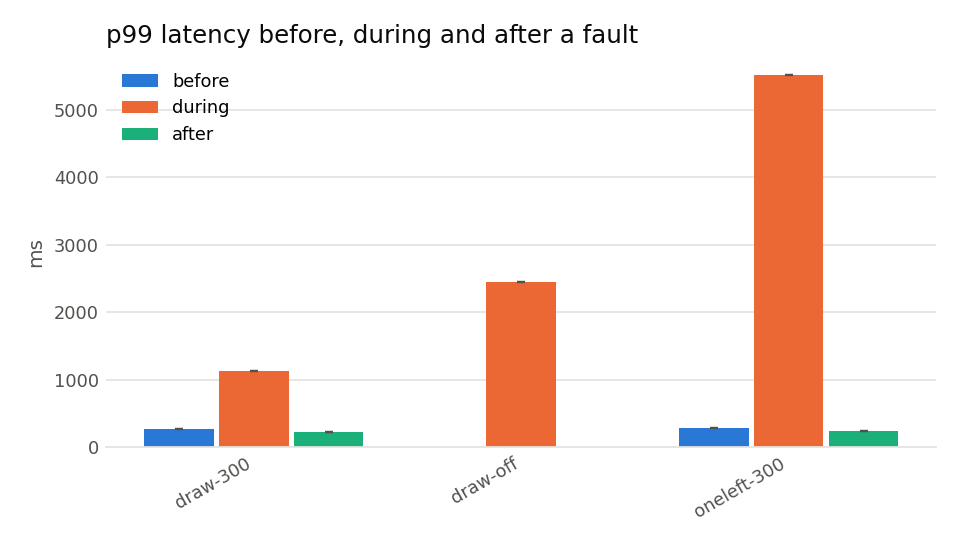
\includegraphics[width=\linewidth]{figures/raft-fault-phases.png}
\par\small (b) p99 around a fault on Raft, from the logs
\end{minipage}
\caption{Results with Raft at \commit{0397d37}. (a) The E1 cells of Table~\ref{tab:raftplan}, mean of 3 runs. (b) The lab guide's T4 with the fault election running (\texttt{draw-300}), T4 with one node off so no draw can go ahead (\texttt{draw-off}, which has no before and after), and T2 with one node killed and one silenced (\texttt{oneleft-300}). Made by \texttt{analysis/analyze.py} from the runs in \texttt{runs/hand/}.}
\label{fig:raft-results}
\end{figure}

\textbf{The throughput ladder.} Table~\ref{tab:ladder} lists the highest fixed rate that held at each build, in the order they were built. Raft rose from 600 to 7,000 reports a second as each limit was fixed, and never reached 10,000.

\begin{table}[!htb]
\centering\small
\caption{Highest offered rate that held, per build, on the six PCs. ``Held'' means every report answered and nobody gave up. One run per step unless stated. The rates with no planning load are not comparable with those with it.}
\label{tab:ladder}
\begin{tabularx}{\linewidth}{@{}P{1.6cm}P{1.6cm}rp{1.7cm}L@{}}
\toprule
Build & Shared log & Held/s & \texttt{plan\_work} & What fell \\
\midrule
\commit{0397d37} & Raft & 600 & 1000 & 800 in 1 of 3 tries and its 5-minute hold; 1,000 in all 4 \\
\commit{4d67039} & Raft & 1,000 & 1000 & 2,000 after about 30 s \\
\commit{0790478} & Raft & 3,000 & 1000 & 5,000 froze, a bug in that build, fixed at \commit{d544a35} \\
\commit{0c9e8fb} & Raft & 7,000 & see note & 10,000: 2,717 answered a second (\dlog{D249}) \\
\commit{cdec322} & rounds & 25,000 & 0 & 30,000: 3,573 gave up (60,000 responders, 3 s detection) \\
\commit{eba4d14} & rounds & 33,000 & 0 & 34,000 started to break; 30,000 held for 5 minutes \\
\commit{eba4d14} & rounds & 10,000 & 1000 & 15,000: all 20 planning threads busy \\
\commit{a7ceb34} & rounds & 30,000 & 0 & held in 5 of 5 runs; 33,000 and 35,000 in 3 of 5 \\
\commit{a7ceb34} & rounds & 12,000 & 1000 & held in 5 of 5 runs; 14,000 in 0 of 5 \\
\bottomrule
\end{tabularx}
\end{table}

The 7,000 row has a caveat: its answers all came, with nobody giving up, but its p99 was 1.2 s, which failed the stricter test used at the time. The folder's run files record its \texttt{plan\_work}, and that value is not copied into the repository.
% CHECK: confirm the plan_work of the f4 runs (analysis/results/f4-stress-summary.txt) from their run.json on client PC 1.

\textbf{The cleanest comparison.} After the switch, Raft was run once more, on the final code, at 10,000 reports a second with 60,000 responders, by setting \texttt{consensus = "raft"} (\texttt{runs/phase1/raft0/10000}). Nothing else changed. Figure~\ref{fig:raft-vs-rounds} sets it beside the same rate on rotating rounds. Raft is one run and rounds five, so the comparison is indicative, but the gap is not small.

\begin{figure}[!htb]
\centering
\begin{tikzpicture}
\begin{axis}[
  ybar, bar width=1.1cm, width=0.62\linewidth, height=5.6cm,
  ymin=0, ymax=11500, ylabel={answered per second},
  symbolic x coords={Raft, Rounds}, xtick=data, enlarge x limits=0.55,
  nodes near coords, nodes near coords style={font=\scriptsize},
  every axis plot/.append style={draw=black!60},
  ytick={0,2500,5000,7500,10000}, scaled y ticks=false, yticklabel style={/pgf/number format/fixed, /pgf/number format/1000 sep={,}, font=\scriptsize},
  title={Offered: 10,000 reports a second, same code}, title style={font=\small},
  axis lines*=left, ymajorgrids, grid style={black!10},
  nodes near coords align={vertical},
  point meta=explicit symbolic,
]
\addplot[fill=nodeblue!55] coordinates {(Raft,4306) [4{,}306] (Rounds,9994) [9{,}994]};
\end{axis}
\end{tikzpicture}
\hspace{0.4cm}
\begin{minipage}[b]{0.3\linewidth}\small
\begin{tabular}{@{}lrr@{}}
\toprule
 & Raft & Rounds \\
\midrule
Runs & 1 & 5 \\
Answered/s & 4,306 & 9,994 \\
Gave up & 341,568 & 0 \\
\bottomrule
\end{tabular}
\vspace{0.8cm}
\end{minipage}
\caption{Raft against rotating rounds on the final code, at the target of 10,000 reports a second. Rounds is \texttt{s0-10000} from the overnight series (Section~\ref{sec:stress}).}
\label{fig:raft-vs-rounds}
\end{figure}

\textbf{The lab guide's tests on both designs.} The same tests ran on Raft and on rounds, with 300 users and \texttt{plan\_work} 1000 (Table~\ref{tab:t1t2}). T1 kills the node that matters most and brings it back; T2 kills one node and silences another, so one node is left for all three client PCs.

\begin{table}[!htb]
\centering\small
\caption{T1 and T2 on both designs. Raft at \commit{0397d37} with 5-minute loads; rounds at \commit{eba4d14} with 3-minute loads.}
\label{tab:t1t2}
\begin{tabularx}{\linewidth}{@{}P{4.2cm}LL@{}}
\toprule
 & Raft & Rotating rounds \\
\midrule
T1: gave up, unaccounted, mismatches & 0, 0, 0 & 0, 0, 0 \\
T1: who takes over & new leader in 778 ms & the other two drop it within 1 s \\
T1: longest time a client PC had no answer & 863 to 867 ms & 251 ms \\
T1: back as a full member & 963 ms after restart & 1.0 s after restart \\
T2: gave up, final digests & 0, equal & 0, equal \\
T2: provisional answers from the lone node & 4,975 & 4,780 \\
T2: later found to differ (responder taken, lost first commit) & 3,908 and 8 & 4,391 and 269 \\
\bottomrule
\end{tabularx}
\end{table}

T1 shows the two designs' failover from different angles. Under Raft, reports still flowed while only the old leader's role was lost, but every commit stopped until the new leader came, about 0.8 s. Under rounds, any surviving node keeps bidding and planning at once, and only its commits wait for the drop at about 1 s, so a client PC waited less. Sections~\ref{sec:faults} and \ref{sec:results} give the full failure results on rounds.

\subsection{What the switch cost}

Removing the leader was not free, and the costs are listed here, beside the gains.

\begin{itemize}
  \item \textbf{Failure detection sets the failover time.} A silent member holds up every round until the others drop it, so a failure costs at least the 1 s detection time, against Raft's 0.8 s new leader.
  \item \textbf{The ordering is the team's own code}, about 1,650 lines in \texttt{rounds.rs}, with no library's users behind it. Its correctness rests on the team's tests and experiments. The first version gave different digests on the lab PCs twice, and each bug was fixed with a test that fails without the fix (\dlog{D252}, \dlog{D257}).
  \item \textbf{Two failures close together stopped commits} in the first version, where Raft would have carried on with two of three. Making the system survive two and three failures took four more decisions (\dlog{D261} to \dlog{D264}), and with all three killed it can still lose a few answers (Section~\ref{sec:limits}).
  \item \textbf{Every node sends every round}, even when idle, so the log costs messages at no load.
\end{itemize}

The gains are the reason these costs are accepted: no node orders the others, the throughput limit moved from 7,000 to 30,000 reports a second without planning and to 12,000 with it, and every member can commit as long as the others are alive.
